%==============================================================================
% Programação Linear
% 25/08/2021
%==============================================================================

\chapter{Programação Linear}

\section{Discussão da Solução Ótima} %-----------------------------------------

Antes de entrarmos na discussão da solução ótima faremos alguns comentários sobre
o \textbf{Método Simplex}.

O Método Simplex faz uso do algorítimo \textbf{Simplex Duas Fases}.
A Fase I é requerida quando após se acrescentar as variáveis de folga e de excesso
às inequações, isto é, passar o problema à forma padrão, não se vislumbra uma
solução básica factível de pronto.
O objetivo da Fase I é obter uma solução básica factível inicial.
A Fase II é o algorítimo propriamente dito, que para começar as iterações requer
uma solução básica factível inicial.
Os problemas cujas restrições são inequações do tipo ``menor ou igual'', e lembrando
que o vetor $ b $ é sempre positivo, têm sempre uma solução básica factível
inicial.
Nos outros casos, em geral, não tem uma solução básica factível inicial, logo,
necessitam de proceder a Fase I.

Para discussão da solução ótima, suporemos que se tem uma solução básica factível
inicial.
Logo, vamos utilizar a Fase II.

Tanto na Fase I, como na Fase II, a cada iteração verifica-se se a solução básica
atual é ótima.
Se é ótima, fim.
Se não é ótima, se vai para o critério de escolha da variável não básica que deve 
ser a candidata para entrar na base.
Escolhida a variável não básica candidata a entrar na base vem o critério da 
variável básica que sairá da base.

Pode ocorrer empate, tanto para a escolha da variável entrante, como para escolha
da que vai sair.
Ditas essas coisas em linhas gerais, vamos aos detalhes.

Voltemos ao sistema de equações,

\begin{align*}
  \min \quad        & z = c_I \inversaA b + \left[c_J - c_I \inversaA A^{J}\right] x_J\\
  \text{s.a.} \quad & x_I + \inversaA A^{J} x_J = \inversaA b \\
                    & x_I, x_J \geq 0
\end{align*}

Na Função Objetivo a parte variável é a segunda parcela do segundo membro,

\[
  \left[ c_J - c_I \inversaA A^{J} \right]  x_J
\]

Suponha que a solução básica atual é ótima.
Isto significa que o valor de $ z $, que é $ c_I \inversaA b $, não tem mais 
como diminuir, ou seja, se algum $ x_j $ (variável não básica) aumentar de valor,
o valor de $ z $ aumentará.
Isto implica que o coeficiente $ \widehat{c}_j $ de $ x_j $ é positivo.
Por outro lado, se todos os $ \widehat{c}_j > 0 $, qualquer variável $ x_j $
que aumentar de valor fará o valor de $ z $ também aumentar, logo, a solução 
atual é ótima.

Conclusão:

\begin{center}
\fbox
{
  \begin{minipage}{0.7\linewidth}
    A solução básica atual é ótima e única se, e somente se, $ \widehat{c}_j > 0 $,
    $ \forall j \in J $.
  \end{minipage}
}
\end{center}

Se a solução básica atual é ótima e algum $ \widehat{c}_j = 0 $, haverá infinitas 
soluções ótimas, pois para cada valor positivo que $ x_j $ assumir corresponderá 
a novos valores das variáveis básicas, mas o valor de $ z $ permanece o mesmo, 
ou seja, $ c_I \inversaA b $, pois $ \widehat{c}_j x_j = 0 $.
Para saber os valores das variáveis básicas para cada valor positivo assumido
por $ x_j $, observe a equação de bloqueio:

\[
  x_I + \widehat{A}^j x_j = \widehat{b}
\]

Agora cabe uma pergunta: \textit{Neste caso há outra solução básica ótima?}
Mais uma vez a resposta é dada pela equação de bloqueio.

Se algum $ \widehat{a}_ij > 0 $, haverá outra solução básica ótima, pois a 
variável básica da linha $ i $ irá para zero quando $ x_j $ aumentar de valor.
Caso haja mais de um $ \widehat{a}_ij > 0 $, as variáveis básicas das respectivas
linhas irão para zero.
Mas, se uma variável atingiu o valor zero, o $ x_j $ não pode mais aumentar de 
valor, caso contrário, a variável básica torna-se-á negativa.
Logo, $ x_j $ será bloqueado quando a primeira variável básica atingir o valor
zero.
O valor de $ x_j $ que faz a variável básica $ x_{B_i} = 0 $ é dado por:

\[
  \frac{\widehat{b}_i}{\widehat{a}_{ij}}  
\]

Assim, se houver mais de uma variável básica indo para zero, deve se escolher
aquela que primeiro atingir zero.
Para isso, calcula-se:

\[
  \min_{i}  
  \left\{\, 
    \frac
    {
      \widehat{b}_i
    }
    {
      \widehat{a}_{ij}
    }; 
    \quad 
    \widehat{a}_{ij} > 0 
  \,\right\}
\]

\begin{obs}
  Se duas ou mais variáveis básicas atingirem zero simultaneamente, estamos 
  diante de uma solução básica degenerada.
  Mas, só uma delas sai da base e $ x_j $ entra no lugar da que saiu.
\end{obs}

O cáculo iterativo para se chegar a nova solução básica é transformar a coluna
$ \widehat{A}^j $ na coluna da matriz identidade que está com a variável básica
que está saindo da base.
Se $ x_{B_i} $ é a variável básica que está saindo da base, o primeiro cálculo
a ser feito é dividir toda linha $ i $ por $ \widehat{a}_{ij} $.
A partir daí, por meio de operações elementares sobre as linhas, é transformar
em zero o $ \widehat{c}_j $ e todos os $ \widehat{a}_{kj} $, com $ k \in I $ e 
$ k \neq i $.
Feito isto, obteve-se a nova solução básica.
Agora, volta-se ao teste de otimalidade.

\section{Montagem do Quadro Simplex} %-----------------------------------------

Toda a discussão sobre a solução ótima e pivoteamento foram realizadas com o P.L.
na forma:

\begin{align*}
  \min        \quad & z = c_I \inversaA b + \left[c_J - c_I \inversaA A^J \right] x_J \\
  \text{s.a.} \quad & x_I + \inversaA A^J x_J = \inversaA b \\
                    & x_I, x_J \geq 0
\end{align*}

Para montagem do quadro, toda expressão que tiver variável colocamos no primeiro
membro das equações, e as constantes, no segundo.
Mas, para manter a discussão sem alterações, sobre o sinal de $ \widehat{c}_J $,
colocamos a F.O. na seguinte forma:

\[
  \left[c_J - c_I \inversaA A^J \right] x_J - z = -c_I \inversaA b
\]

E o quadro do Simplex é o seguinte:

\begin{table}[!htbp]
  \centering
  \begin{tabular}{c|ccc|c}
    Min         & $x_I$        & $x_J$                       &  $z$  & \\ \hline
    Var. Bás.   & $0$          & $c_J - c_I \inversaA A^{J}$ & $-1$  & $-c_I \inversaA b$\\ \hline
    $x_I$       & $\mathbb{I}$ & $\inversaA A^J$             & $0$   & $\inversaA b$ \\ \hline
                &              & $x_I, x_J \geq 0$           &       &
  \end{tabular}
\end{table}

Ou fazendo uso da notação simplificada:

\begin{table}[!htbp]
  \centering
  \begin{tabular}{c|ccc|c}
    Min       & $x_I$        & $x_J$           & $z$  & \\ \hline
    Var. Bás. & $0$          & $\widehat{c}_J$ & $-1$ & $-c_I \inversaA b$ \\ \hline
    $x_I$     & $\mathbb{I}$ & $\widehat{A}^J$ & $0$  & $\widehat{b}$ \\ \hline
              &              & $x_I, x_J$      &      &
  \end{tabular}
\end{table}

Na prática, na primeira linha, as variáveis são dispostas na ordem crescente dos
índices; e, na última linha, não colocamos.

Os procedimentos e discussões sobre a solução ótima são os mesmso tanto para a 
Fase I, como para a Fase II.

Vejamos um exemplo que não requer a Fase I.

\begin{exemplo}
  Resolva o P.L. abaixo:
  \begin{align*}
    \min        \quad & z = -3 x_1 + 5 x_2 - 2 x_3 \\
    \text{s.a.} \quad & 
                        \begin{aligned}[t]
                          2 x_1 + 2 x_2 + 4 x_3 &\leq 12 \\
                          - x_1 + 3 x_2 + 2 x_3 &\leq 6  \\
                          2 x_1 + 4 x_2 -   x_3 &\leq 4
                        \end{aligned}\\
                      & x_1, x_2, x_3 \geq 0.
  \end{align*}
\end{exemplo}

Primeiro passa o problema para forma padrão, acrescentando-se as variáveis de 
folga.

\begin{align*}
  \min        \quad & z = -3 x_1 + 5 x_2 - 2 x_3 \\
  \text{s.a.} \quad & 
                      \begin{aligned}[t]
                        2 x_1 + 2 x_2 + 4 x_3 + x_4 \phantom{+ x_5 + x_6} &= 12 \\
                        - x_1 + 3 x_2 + 2 x_3 \phantom{+ x_4} + x_5 \phantom{+ x_6}&= 6  \\
                        2 x_1 + 4 x_2 -   x_3 \phantom{+ x_4 + x_5} + x_6 &= 4
                      \end{aligned}\\
                    & x_1, x_2, x_3, x_4, x_5 \geq 0.
\end{align*}

Note que há uma solução básica factível inicial: 
\begin{itemize}
  \item \textbf{Variáveis Básicas:} $ x = 12, x_5 = 6 \text{ e } x = 4 $;
  \item \textbf{Variáveis não Básicas:} $ x_1 = x_2 = x_3 = 0$;
  \item \textbf{Valor de F.O.}: $ z = 0 $.
\end{itemize}

Montando o quadro Simplex:

\begin{table}[!htbp]
  \centering
  \begin{tabular}{c|ccccccc|c}
    Min             & $\setaEntra{1}$   & $x_2$ & $x_3$ & $x_4$ & $x_5$ & $x_6$ & $z$  &      \\ \hline
    Var. Bás.       & $-3$              & $5$   & $-2$  & $0$   & $0$   & $0$   & $-1$ & $0$  \\ \hline           
    $x_4$           & $ 2$              & $2$   & $4$   & $1$   & $0$   & $0$   & $0$  & $12$ \\
    $x_5$           & $-1$              & $3$   & $2$   & $0$   & $1$   & $0$   & $0$  & $6$  \\
    $\setaSai{6}$   & $\circulo{2}$     & $4$   & $-1$  & $0$   & $0$   & $1$   & $0$  & $4$
  \end{tabular}
\end{table}

Neste caso, em que as inequações são todos do tipo ``$\leq$'', o quadro sempre está
preparado, istó é, pronto para discussão se a solução  básica atual é ótima ou
não.

Há dois $\widehat{c} < 0$, o que indica que a solução básica atual não é ótima 
($\widehat{c}_7 = -3$ e $\widehat{c}_3 = -2$).
O mais negativo corresponde à variável não básica que deve ser a candidata a 
entrar na base.
Logo, $ x_1 $ é a candidata a entrar  na base.
Agora, examinaremos o $ \widehat{A}^{1} $.

\[
  \widehat{A}^{1} = 
    \begin{bmatrix}
      2 \\
      -1 \\
      2
    \end{bmatrix}
\]

Como há elementos positivos, há outra solução básica factível que melhora a F.O.
($\widehat{a}_{11} = 2$ e $\widehat{a}_{31} = 2$).

A equação de bloqueio é 
\[
  \begin{bmatrix}
    x_4 \\
    x_5 \\
    x_6
  \end{bmatrix}  
  +
  \begin{bmatrix}
    2 \\
    -1\\
    2
  \end{bmatrix}
  = 
  \begin{bmatrix}
    12 \\
    6 \\
    4
  \end{bmatrix},
\]
 e o cálculo prático para se saber que variável  básica sai da base é 
 \[
   \Min_{i} \left\{ \frac{\widehat{b}_i}{\widehat{a}_{ij}}; \;\; \widehat{a}_{ij} > 0 \right\}
 \]

 Assim, tem-se o seguinte:
 \[
   \Min\left\{\frac{12}{2}, \frac{4}{2}\right\}  = \frac{4}{2} = 2.
 \]

 Significa que $ x_6 $ deve sair da base, e $ x_1 $ entra na base com valor 2.
 
 Observe: se $ x_1 = 2 $, então $ x_6 = 0, x_4 = 8 \text{ e } x_5 = 8 $.

 A coluna $ \widehat{A}^{1} $ deve ser transformada na coluna 
 \[
   \begin{bmatrix} 
    0 \\ 
    0 \\ 
    1 
   \end{bmatrix} 
\] 
que é a atual coluna de $ x_6 $.

O novo quadro é:

\begin{table}[!htbp]
  \centering
  \begin{tabular}{c|ccccccc|c}
    Min           & $x_1$ & $x_2$ & $\setaEntra{3}$ & $x_4$ & $x_5$ & $x_6$ & $z$  &     \\ \hline
    Var. Bás.     & $0$   & $11$  & $-7/2$          & $0$   & $0$   & $3/2$ & $-1$ & $6$ \\ \hline
    $\setaSai{4}$ & $0$   & $-2$  & $\circulo{5}$   & $1$   & $0$   & $-1$  & $0$  & $8$ \\
    $x_5$         & $0$   & $5$   & $3/2$           & $0$   & $1$   & $1/2$ & $0$  & $8$ \\
    $x_1$         & $1$   & $2$   & $-1/2$          & $0$   & $0$   & $1/2$ & $0$  & $2$ 
  \end{tabular}
\end{table}

A solução básica atual não é ótima: $ \widehat{c}_3 = -7/2 $.
Único negativo, logo, $ x_3 $ é camdidato a entrar na base.

O elemento do encontro da coluna da variável que entra com a linha da variável 
que sai é chamado \textbf{pivô}.
Ele é que será transformado em ``1'' e todos os cálculos são realizados por meio 
dele.

Da \textbf{Equação de Bloqueio} 
\[
  \begin{bmatrix}
    x_4 \\
    x_5 \\
    x_1
  \end{bmatrix}  
  + \begin{bmatrix}
    5    \\
    3/2  \\
    -1/2 \\
  \end{bmatrix}
  = 
  \begin{bmatrix}
    8 \\
    8 \\
    2
  \end{bmatrix}
\]
se retira o cálculo prático, do qual se obtém duas informações:
\begin{enumerate}
  \item[(i)] com que valor $ x_3 $ \textbf{entra};
  \item[(ii)] e que variável \textbf{sai} da base.
\end{enumerate}

Como
\[
  Min\left\{\frac{8}{5}, \frac{8}{3/2}\right\}  = \frac{8}{5},
\]
logo, $x_4$ sai da base.

\begin{table*}[!htbp]
  \centering
  \begin{tabular}{c|ccccccc|c}
    Min       & $x_1$ & $x_2$  & $x_3$ & $x_4$   & $x_5$ & $x_6$  & $z$  &        \\ \hline
    Var. Bás. & $0$   & $48/5$ & $0$   & $7/10$  & $0$   & $4/5$  & $-1$ & $58/5$ \\ \hline 
    $x_3$     & $0$   & $-2/5$ & $1$   & $1/5$   & $0$   & $-1/5$ & $0$  & $8/5$  \\
    $x_5$     & $0$   & $28/5$ & $0$   & $-3/10$ & $1$   & $4/5$  & $0$  & $28/5$ \\
    $x_1$     & $1$   & $9/5$  & $0$   & $1/10$  & $0$   & $2/5$  & $0$  & $14/5$ 
  \end{tabular}
\end{table*}

Todos os $ \widehat{c}_J > 0 $, logo a solução básica atual é ótima e única.

\begin{itemize}
  \item $ \widehat{c}_2 = 48/5, \widehat{c}_4 = 7/10 \;\text{ e }\; \widehat{c}_6 = 4/5 $
  \item o valor ótimo de $ z $ é $ -58/5 $
  \item variáveis básicas: $ x_3 = 8/5, x_5 = 28/5 \;\text{ e }\; x_1 = 14/5 $
  \item variáveis não básicas: $ x_2 = x_4 = x_6 = 0 $
\end{itemize}

\section{Fase I} %-------------------------------------------------------------

\subsection{Procedimentos da Fase I}

\begin{enumerate}
  \item Abandone temporariamente a F.O. do problema;
  \item Crie uma F.O. artificial para ser minimizada e definida pela soma das 
        variáveis artificiais que serão adicionadas às restrições com o problema
        já na forma padrão;
  \item Adicione uma variável na equação que não tiver uma variável básica 
        factível.
        Essa variável adicionada não pertence ao problema; é uma variável 
        artificial;
  \item Monte o quadro Simplex;
  \item Prepare o quadro;
  \item Proceda como na Fase II;
  \item 
   \begin{enumerate}
     \item Se ao chegar na solução ótima a F.O. artificial tiver valor nulo, o 
           problema original é factível.
           Abandone a F.O. e extraia a solução básica encontrada para montar o
           quadro Simplex para Fase II.
     \item Se ao chegar na solução ótima o valor da a F.O. for \textit{diferente} 
           de zero, o problema original é \textit{infactível}, isto é, o conjunto
           das soluções factíveis é vazio.           
   \end{enumerate}
\end{enumerate}

Vejamos dois exemplos: um em que o problema é infactível, e outro, factível.

\begin{exemplo}
  Encontre, se possível, uma solução básica factível para o P.L. abaixo:

  \begin{align*}
    \max        \quad & z = 6 x_1 + 8 x_2 \\
    \text{s.a.} \quad & 
                        \begin{aligned}[t]
                          -2 x_1 + 3 x_2 &\geq 6 \\
                           2 x_1 - 3 x_2 &\geq 4 \\
                           3 x_1 + 2 x_2 &\leq 8
                        \end{aligned}\\
                      & x_1, x_2 \geq 0
  \end{align*}
\end{exemplo}

Passando o problema para forma padrão, não se obtém uma solução básica factível
inicial.
Logo, é necessário a Fase I.

\begin{align*}
  \max        \quad & z = 6 x_1 + 8 x_2 \\
  \text{s.a.} \quad &
                      \begin{aligned}[t]
                        -2 x_1 + 3 x_2 - x_3 \phantom{- x_4 + x_5}           &= 6 \\
                         2 x_1 - 3 x_2 \phantom{- x_3} - x_4 \phantom{+ x_5} &= 4 \\
                         3 x_1 + 2 x_2 \phantom{- x_3 - x_4} + x_5           &= 8
                      \end{aligned}\\
                    & x_1, x_2, x_3, x_4, x_5 \geq 0
\end{align*}

A solução básica que se é infactível.
$ x_3 = -6, x_4 = -4 \;\text{ e } $ $ x_5 = 8 $ são as variáveis básicas, e 
$ x_1 = x_2 = 0 $, são as não básicas.

\textit{Fase I}

\begin{align*}
  \max        \quad & w = x_6 + x_7 \\
  \text{s.a.} \quad &
                      \begin{aligned}[t]
                        -2 x_1 + 3 x_2 - x_3 \phantom{- x_4 + x_5} + x_6 \phantom{+ x_7} &= 6 \\
                         2 x_1 - 3 x_2 \phantom{- x_3} - x_4 \phantom{+ x_5 + x_6} + x_7 &= 4 \\
                         3 x_1 + 2 x_2 \phantom{- x_3 - x_4} + x_5 \phantom{+ x_6 + x_7} &= 8
                      \end{aligned}\\
                    & x_1, x_2, x_3, x_4, x_5, x_6, x_7 \geq 0
\end{align*}

Com a adição das variáveis artificiais $ x_6 $ e $ x_7 $, obtém-se uma solução
básica factível, mas ela é artificial; não pertence ao problema original.
A solução básica factível artificial é $ x_6 = 6, x_7 = 4 \;\text{ e }\; x_5 = 8 $,
as variáveis básicas, $ x_1 = x_2 = x_3 = x_4 = 0 $, as não básicas e $ w = 10 $.

\newpage

\begin{table}[!htbp]
  \centering
  \caption{Montando o quadro}
  \begin{tabular}{c|cccccccc|c}
    Min       & $x_1$ & $x_2$ & $x_3$ & $x_4$ & $x_5$ & $x_6$ & $x_7$ & $w$ &  \\
    \hline
    Var. Bás. & $0$     & $0$     & $0$     & $0$     & $0$     & $1$     & $1$     & $-1$  & $0$  \\
    \hline
    $x_6$     & $-2$    &  $3$    & $-1$    &  $0$    & $0$     & $1$     & $0$     & $0$   & $6$ \\ 
    $x_7$     &  $2$    & $-3$    &  $0$    & $-1$    & $0$     & $0$     & $1$     & $0$   & $4$ \\
    $x_5$     &  $3$    &  $2$    &  $0$    &  $0$    & $1$     & $0$     & $0$     & $0$   & $8$
  \end{tabular}
\end{table}

O quadro não está preparado.

\begin{table}[!htbp]
  \centering
  \caption{Quadro Preparado}
  \begin{tabular}{c|cccccccc|c}
    Min       & $x_1$ & $x_2$ & $x_3$ & $x_4$ & $x_5$ & $x_6$ & $x_7$ & $w$ &  \\
    \hline
    Var. Bás. & 0     & 0     & 1     & 1     & 0     & 0     & 0     & -1  & -10 \\
    \hline
    $x_6$     & -2    &  3    & -1    &  0    & 0     & 1     & 0     & 0   & 6 \\ 
    $x_7$     & 2     & -3    &  0    & -1    & 0     & 0     & 1     & 0   & 4 \\
    $x_5$     & 3     &  2    &  0    &  0    & 1     & 0     & 0     & 0   & 8
  \end{tabular}
\end{table}

O quadro está preparado, mas apresenta a solução com a $ F.O. \neq 0 $.
Portanto, o problema original é infactível.
Note que os $ \widehat{c}_j \geq 0 $, isto é, $ \widehat{c}_1 = 0, 
\widehat{c}_2 = 0, \widehat{c}_3 = 1 \;\text{ e }\; \widehat{c} = 1$.

A Figura~\ref{fig:retas} mostra que o conjunto das soluções é vazio.

\begin{figure}[!h]
  \centering
  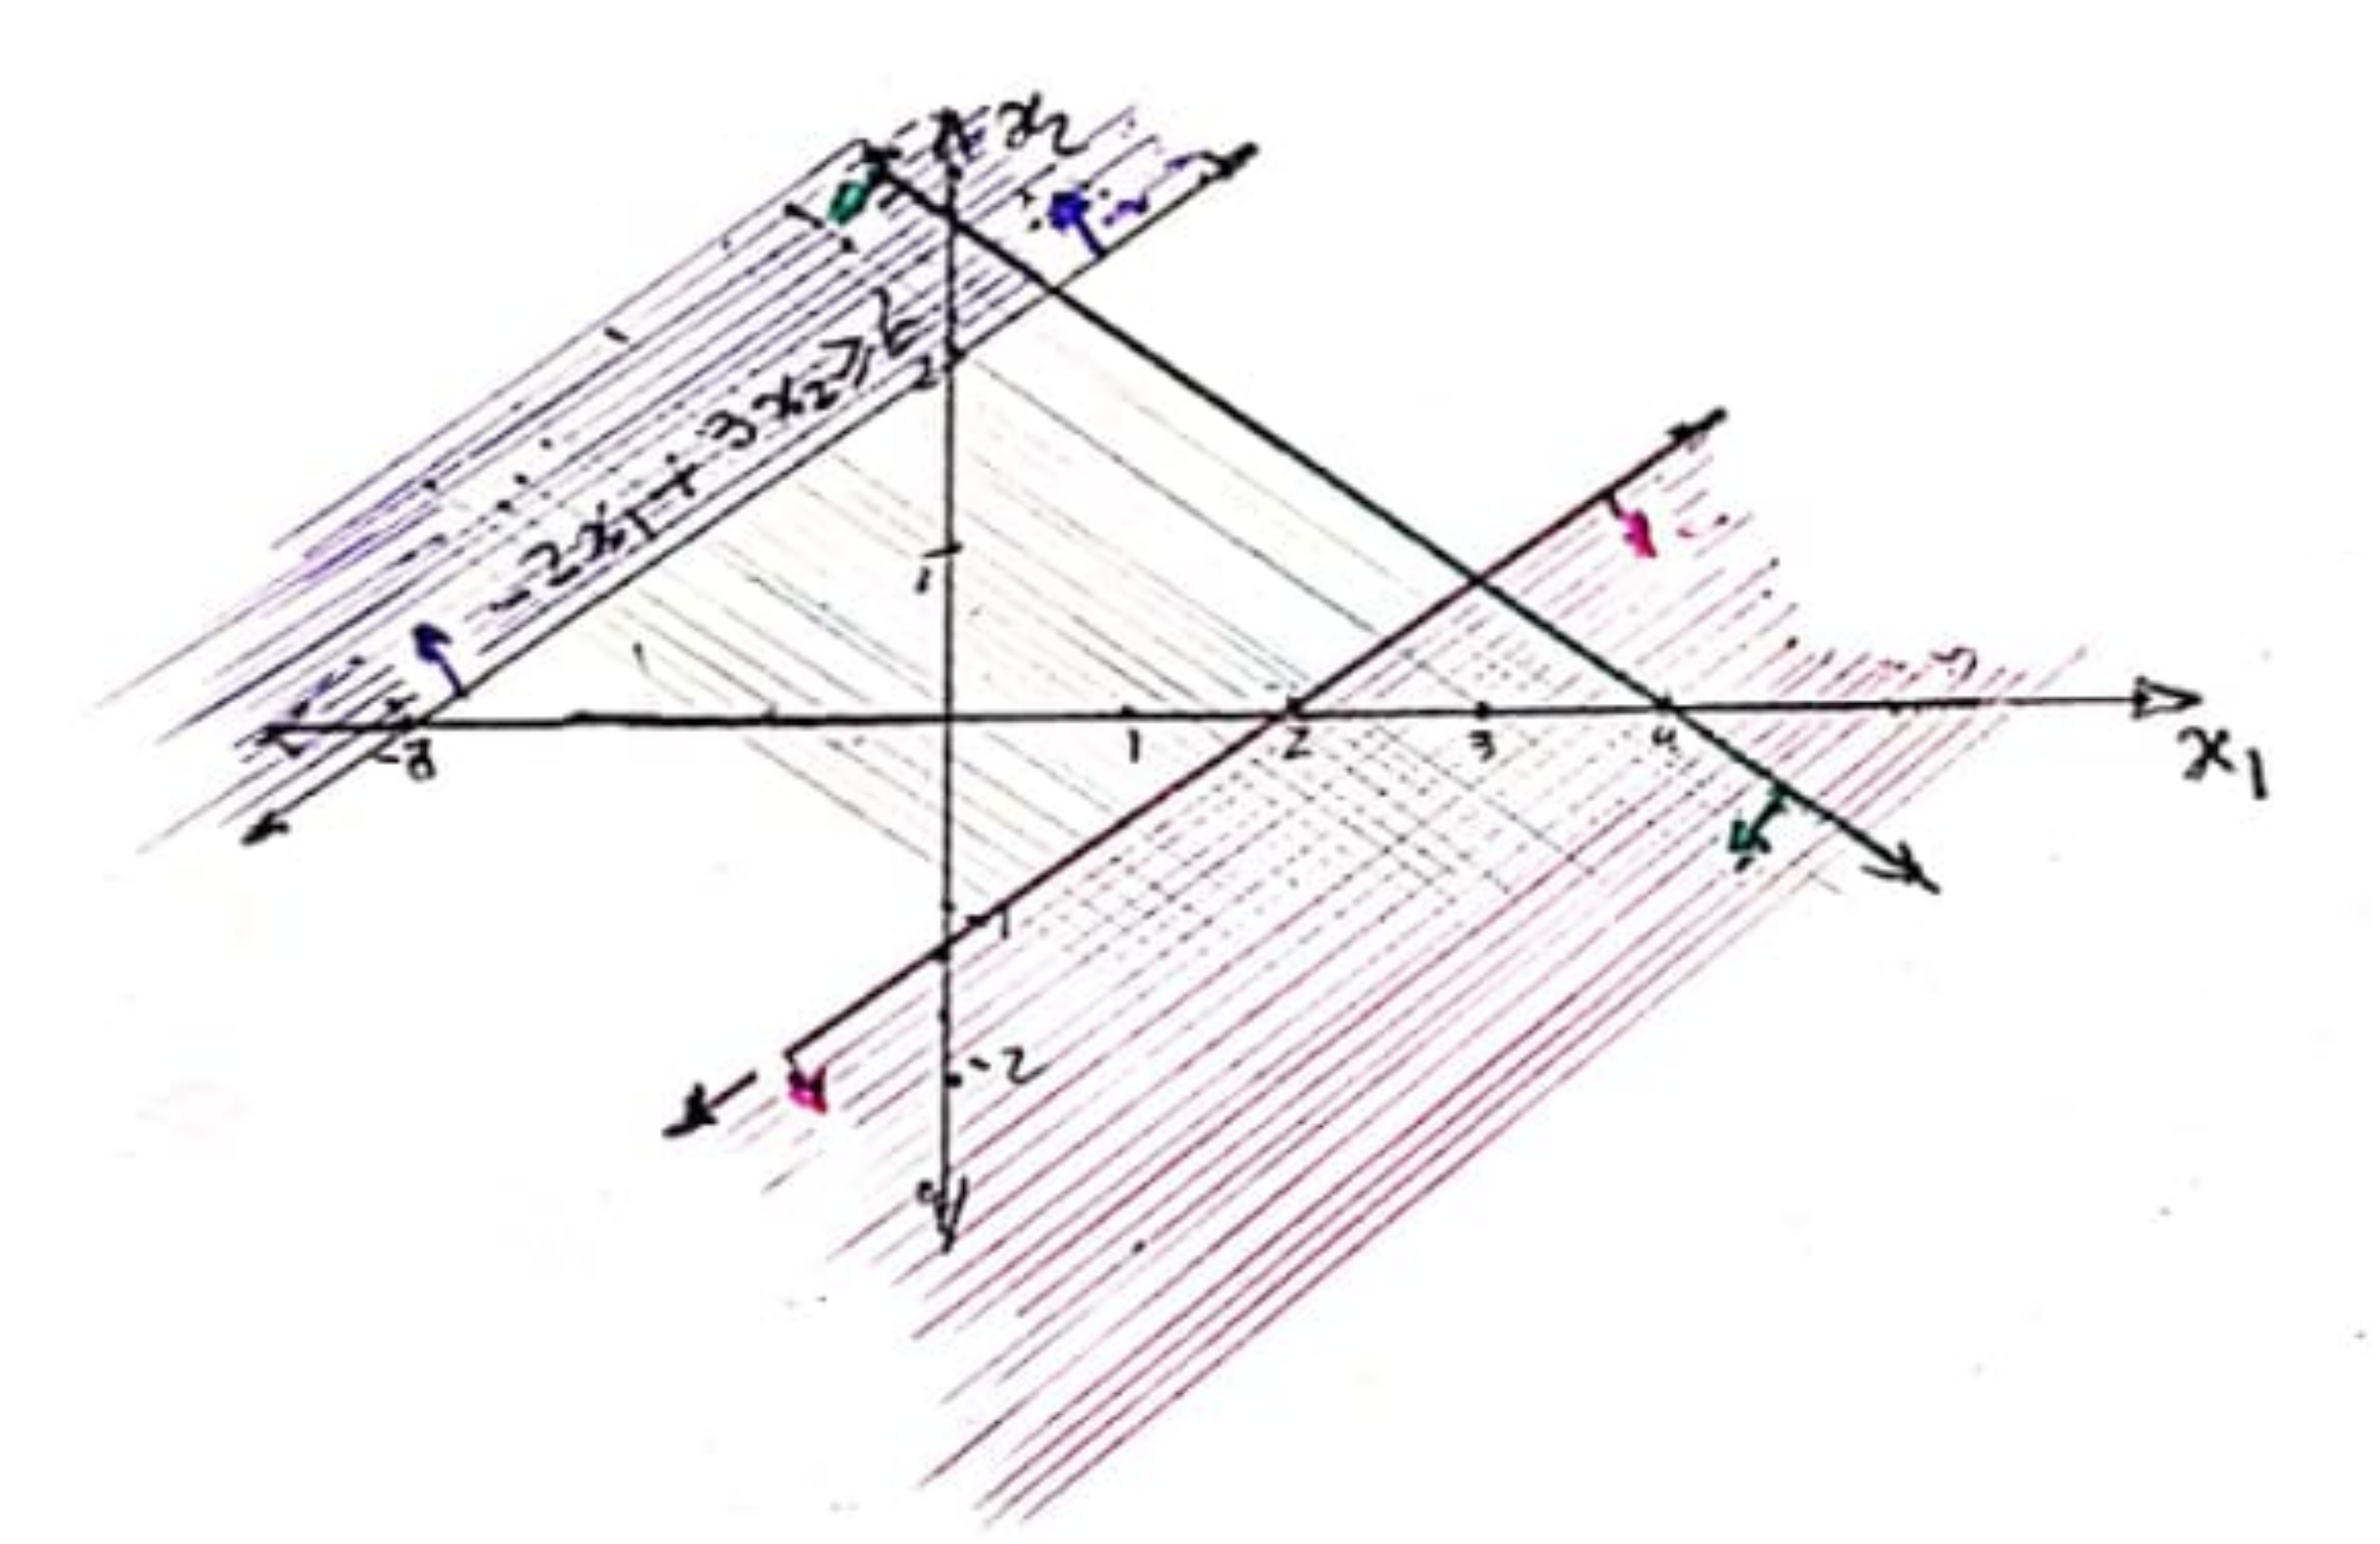
\includegraphics[width = 0.9\linewidth]{retas}
  \caption{Note que não há região alguma comum às três inequações.}
  \label{fig:retas}
\end{figure}

\newpage

\begin{exemplo}
Aplique a Fase I para obter uma solução básica factível do problema abaixo, 
deixando no final o quadro preparado para a Fase II.

\begin{align*}
  \max        \quad & z = 4 x_1 + 3 x_2  \\
  \text{s.a.} \quad & 
                      \begin{aligned}[t]
                          x_1 + 5 x_2 &\geq 5  \\
                        3 x_1 + 4 x_2 &\leq 12 \\
                        2 x_1 +   x_2 &\geq 4
                      \end{aligned}\\
                    & x_1, x_2 \geq 0
\end{align*}
\end{exemplo}

Passando o problema à forma padrão:

\begin{align*}
  \max        \quad & z = 4 x_1 + 3 x_2 \\
  \text{s.a.} \quad & 
                      \begin{aligned}[t]
                          x_1 + 5 x_2 - x_3 \phantom{+ x_4 - x_5}           &= 5  \\
                        3 x_1 + 4 x_2 \phantom{- x_3} + x_4 \phantom{- x_5} &= 12 \\
                        2 x_1 +   x_2 \phantom{- x_3 + x_4} - x_5           &= 4
                      \end{aligned}\\
                    & x_1, x_2, x_3, x_4, x_5 \geq 0
\end{align*}

Observe que a solução básica que se tem é infactível:
\begin{itemize}
  \item $ x_3 = -5, x_4 = 12 \;\text{ e }\; x_5 = -4 $ são as variáveis básicas;
  \item $ x_1 = x_2 = 0 $ são as não básicas.
\end{itemize}

\textit{Fase I:}

\begin{align*}
  \min        \quad & w = x_6 + x_7 \\
  \text{s.a.} \quad & 
                      \begin{aligned}[t]
                         x_1 + 5 x_2 - x_3 \phantom{+ x_4 - x_5} + x_6 \phantom{+ x_7} &= 5 \\
                       3 x_1 + 4 x_2 \phantom{- x_3} + x_4 \phantom{- x_5 + x_6 + x_7} &= 12 \\
                       2 x_1 +   x_2 \phantom{- x_3 + x_4} - x_5 \phantom{+ x_6} + x_7 &= 4
                      \end{aligned}\\
                    & x_1, x_2, x_3, x_4, x_5, x_6, x_7 \geq 0
\end{align*}

Agora tem-se uma solução básica factível, mas é artificial, não pertence ao 
problema original.
\begin{itemize}
  \item Variáveis Básicas: $ x_6 = 5, x_4 = 12\;\text{ e }\; x_7 = 4 $;
  \item Variáveis não Básicas: $ x_1 = x_2 = x_3 = x_5 = 0 $;
  \item Valor de $w$: $ w = 9 $.
\end{itemize}

\newpage

Montando o quadro

\begin{table}[!htbp]
  \centering
  \begin{tabular}{c|cccccccc|c}
    Min       & $x_1$ & $x_2$ & $x_3$ & $x_4$ & $x_5$ & $x_6$ & $x_7$ & $w$ &    \\ \hline 
    Var. Bás. & 0     & 0     & 0     & 0     & 0     & 1     & 1     & -1  & 0  \\ \hline
    $x_6$     & 1     & 5     & -1    & 0     & 0     & 1     & 0     & 0   & 5  \\
    $x_4$     & 3     & 4     & 0     & 1     & 0     & 0     & 0     & 0   & 12 \\
    $x_7$     & 2     & 1     & 0     & 0     & -1    & 0     & 1     & 0   & 4  
  \end{tabular}
\end{table}

O quadro não está preparado.

\begin{table}[!htbp]
  \centering
  \caption{Quadro Preparado}
  \begin{tabular}{c|cccccccc|c}
    Min           & $x_1$ & $\setaEntra{2}$ & $x_3$ & $x_4$ & $x_5$ & $x_6$ & $x_7$ & $w$ &    \\ 
    \hline 
    Var. Bás.     & -3    & -6              & 1     & 0     & 1     & 0     & 0     & -1  & -9  \\ 
    \hline
    $\setaSai{6}$ & 1     & \circulo{5}     & -1    & 0     & 0     & 1     & 0     & 0   & 5  \\
    $x_4$         & 3     & 4               & 0     & 1     & 0     & 0     & 0     & 0   & 12 \\
    $x_7$         & 2     & 1               & 0     & 0     & -1    & 0     & 1     & 0   & 4
  \end{tabular}
\end{table}

Como há $ \widehat{c}_j < 0 $, a solução básica atual não é ótima.
O mais negativo é $ \widehat{c}_2 $, isto é, $-6$.
Assim, $ x_2 $ é candidato a entrar na base.
A equação de bloqueio fornece a informação que variável básica sairá da base.

\[
  x_I + \widehat{A}^2 x_2 = \widehat{b}, 
  \quad 
  \text{ou seja}, 
  \quad
  \begin{bmatrix}
    x_6 \\
    x_4 \\
    x_7
  \end{bmatrix}
  + 
  \begin{bmatrix}
    5 \\
    4 \\
    1  
  \end{bmatrix}
  x_2
  =
  \begin{bmatrix}
    5  \\
    12 \\
    4
  \end{bmatrix}
\]

Cálculo prático: $\min \left\{\,\frac{\widehat{b}_i}{\widehat{a}_{ij}};\;\; \widehat{a}_{ij} > 0\,\right\}$,
ou seja, 
\[
  \min \left\{\frac{5}{5}, \frac{12}{4}, \frac{4}{1}\right\} =\frac{5}{5} = 1
\]
Isso implica que $ x_6 $ sai da base e $ x_2 $ entra na base com valor $1$.

\begin{table}[!htbp]
  \centering
  \begin{tabular}{c|cccccccc|c}
    Min           & $\setaEntra{1}$ & $x_2$ & $x_3$ & $x_4$ & $x_5$ & $x_6$ & $x_7$ & $w$ &    \\ \hline 
    Var. Bás.     & -9/5            & 0     & -1/5  & 0     & 1     & 6/5   & 0     & -1  & -3 \\ \hline
    $x_2$         & 1/5             & 1     & -1/5  & 0     & 0     & 1/5   & 0     & 0   & 1  \\
    $x_4$         & 11/5            & 0     & 4/5   & 1     & 0     & -4/5  & 0     & 0   & 8  \\
    $\setaSai{7}$ & \circulo{9/5}   & 0     & 1/5   & 0     & -1    & -1/5  & 1     & 0   & 3
  \end{tabular}
\end{table}

A solução básica atual não é ótima, pois há $ \widehat{c}_j < 0 $ e o mais 
negativo é $ \widehat{c}_1 = -9/5 $.
Pela equação de bloqueio, $ x_I + \widehat{A}^{1}x_1 = \widehat{b} $, ou seja,
\[
  \begin{bmatrix}
    x_2 \\ x_4 \\ x_7
  \end{bmatrix} 
  +
  \begin{bmatrix}
    1/5 \\ 11/5 \\ 9/5 
  \end{bmatrix}
  x_1
  =
  \begin{bmatrix}
    1 \\ 8 \\ 3
  \end{bmatrix}.
\]

Note que, quando $ x_1 $ aumenta de valor, todas as variáveis básicas vão para
zero e quando $ x_1 = 5/3 $, $ x_7 = 0 $, $ x_2 = 5 $ e $ x_4 = 40/11 $.

Assim, $ x_7 $ sai da base.

\begin{table}[!htbp]
  \centering
  \begin{tabular}{c|cccccccc|c}
    Min       & $x_1$ & $x_2$ & $x_3$ & $x_4$ & $x_5$ & $x_6$ & $x_7$ & $w$ &      \\ \hline 
    Var. Bás. & 0     & 0     & 0     & 0     & 0     & 1     & 1     & -1  & 0    \\ \hline
    $x_2$     & 0     & 1     & -2/9  & 0     & 1/9   & 2/9   & -1/9  & 0   & 2/3  \\
    $x_4$     & 0     & 0     & 5/9   & 1     & 11/9  & -5/9  & -11/9 & 0   & 13/3 \\
    $x_1$     & 1     & 0     & 1/9   & 0     & -5/9  & -1/9  & 5/9   & 0   & 5/3
  \end{tabular}
\end{table}

Note que todos os $ \widehat{c}_j \geq 0 $, logo, a solução atual é ótima e como
como $ w = 0 $, o problema original é factível.
A solução básica atual é uma solução do problema original.
Fim da Fase I.
A Figura~\ref{fig:faseI} mostra o caminho da Fase I.

\begin{figure}[!htbp]
  \centering
  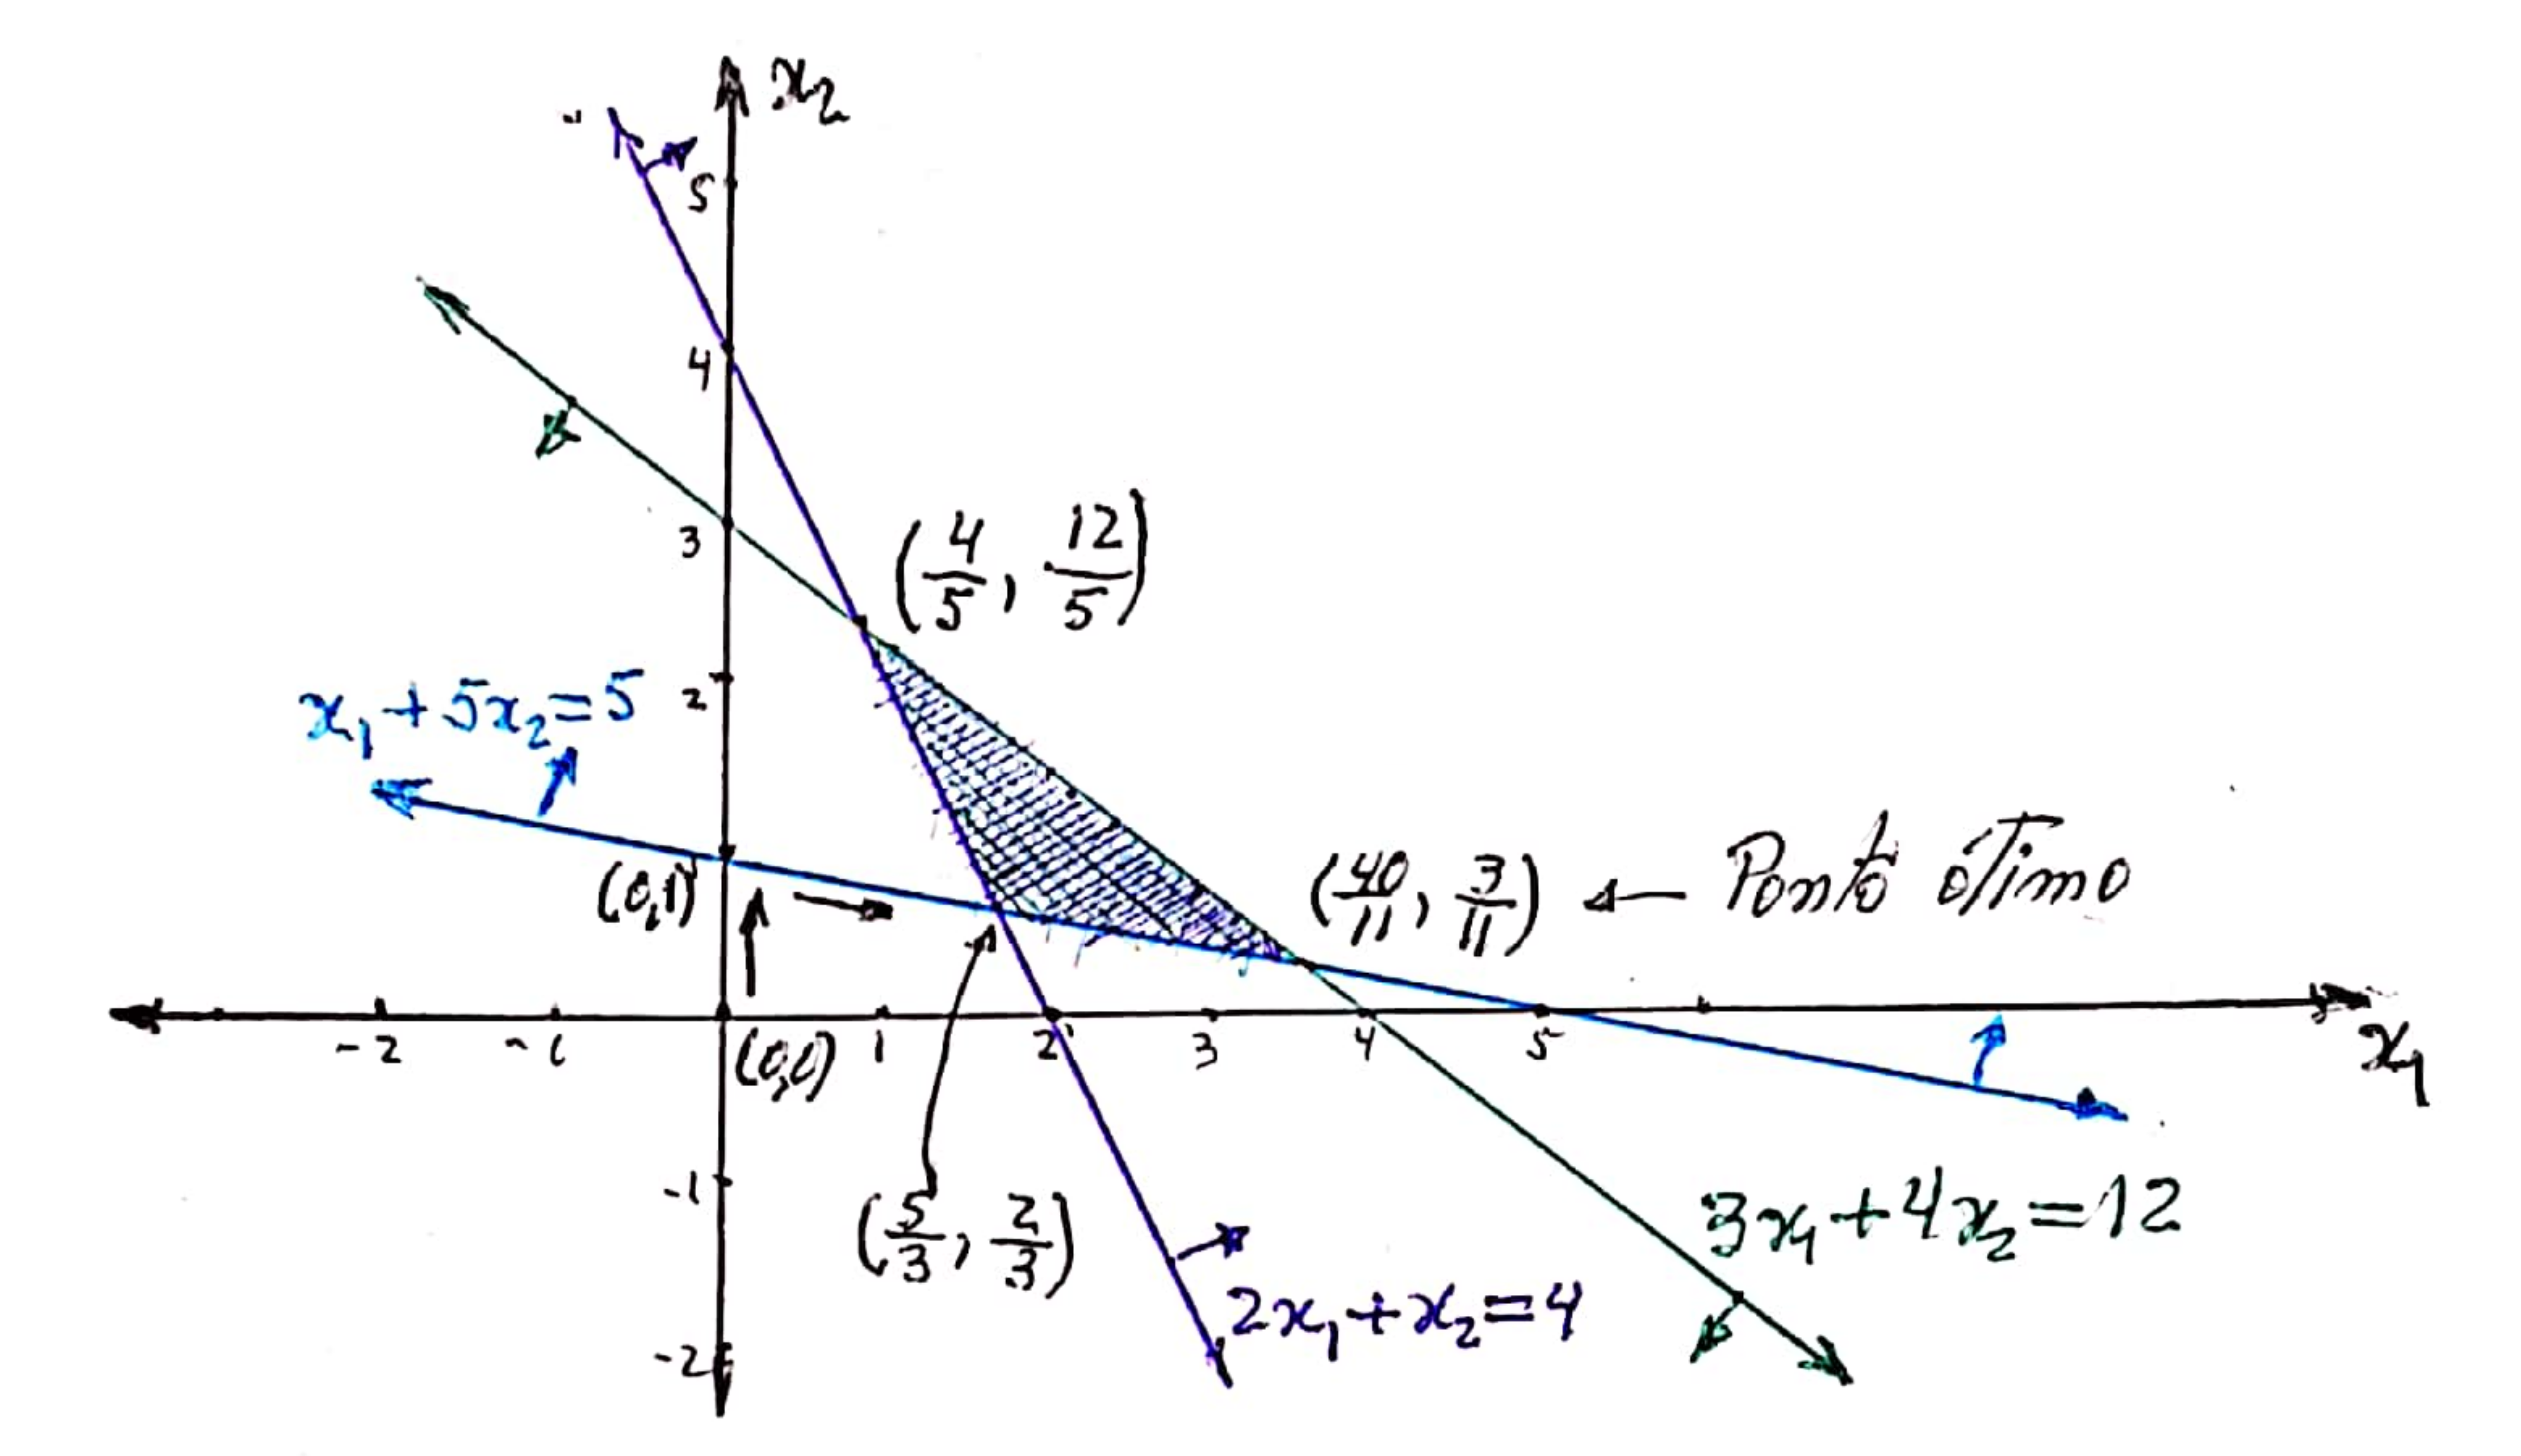
\includegraphics[width = 0.7\linewidth]{faseI.png}
  \caption{O caminho seguido pela Fase I}
  \label{fig:faseI}
\end{figure}

A sequência é $ (0, 0) \to (0, 1) \to \left(5/3, 2/3\right) $.
As soluções básicas correspondes aos pontos $ (0, 0) $ e $ (0, 1) $ são 
infactíveis.

Apenas as soluções básicas factíveis são pontos extremos.

\begin{table}[!htbp]
  \centering
  \caption{Foi colocado o transposto para ocupar menos espaço}
  \begin{tabular}{cl}
    \toprule
    \textbf{Ponto extremo} & \textbf{Solução Básica Factível}\\
    \midrule
    $\left(\frac{5}{3}, \frac{2}{5}\right)$    & $\left[\frac{5}{3}, \frac{2}{5}, 0, \frac{13}{3}, 0 \right]^t$ \\
    $\left(\frac{40}{11}, \frac{3}{11}\right)$ & $\left[\frac{40}{11}, \frac{3}{11}, 0, 0, \frac{39}{11} \right]^t$ \\
    $\left(\frac{4}{5}, \frac{12}{5}\right)$   & $\left[\frac{4}{5}, \frac{12}{5}, \frac{64}{5}, 0, 0 \right]^t$ \\
    \bottomrule
  \end{tabular}
\end{table}

Passemos à Fase II.

\begin{table}[!htbp]
  \centering
  \caption{O quadro não está preparado}
  \begin{tabular}{c|cccccc|c}
    Max       & $x_1$ & $x_2$ & $x_3$ & $x_4$ & $x_5$ & $z$ &      \\ \hline
    Var. Bás. & 4     & 3     & 0     & 0     & 0     & -1  & 0    \\ \hline
    $x_2$     & 0     & 1     & -2/9  & 0     & 1/9   & 0   & 2/3  \\
    $x_4$     & 0     & 0     & 5/9   & 1     & 11/9  & 0   & 13/3 \\
    $x_1$     & 1     & 0     & 1/9   & 0     & -5/9  & 0   & 5/3
  \end{tabular}
\end{table}

O próximo quadro está preparado.

\begin{table}[!htbp]
  \centering
  \caption{O quadro não está preparado}
  \begin{tabular}{c|cccccc|c}
    Max           & $x_1$ & $x_2$ & $x_3$ & $x_4$ & $\setaEntra{5}$ & $z$ &       \\ \hline
    Var. Bás.     & 0     & 0     &  2/9  & 0     & 17/9            & -1  & -26/3 \\ \hline
    $x_2$         & 0     & 1     & -2/9  & 0     &  1/9            & 0   &  2/3  \\
    $\setaSai{4}$ & 0     & 0     &  5/9  & 1     & \circulo{11/9}  & 0   &  13/3 \\
    $x_1$         & 1     & 0     &  1/9  & 0     & -5/9            & 0   &  5/3
  \end{tabular}
\end{table}

A solução básica atual não é ótima; existe $ \widehat{c}_j > 0 $ e o maior valor
é $ \widehat{c}_5 = 17/9 $.

$ \widehat{A}^{5} $ tem elementos positivos, logo, há outra solução básica que
melhora o valor da F.O.

\[
  \widehat{A}^{5} =
  \begin{bmatrix}
    \widehat{a}_{15} \\
    \widehat{a}_{25} \\
    \widehat{a}_{35}
  \end{bmatrix} 
  =
  \begin{bmatrix}
     1/9  \\
     11/9 \\
    -5/9
  \end{bmatrix} .
\]

O cálculo prático $\min \left\{\,\frac{\widehat{b}_i}{\widehat{a}_{ij}};\;\; \widehat{a}_{ij} > 0\,\right\}$,
ou seja, 
\[
  \min \left\{\frac{2/3}{1/9}, \frac{13/3}{11/9}\right\}  
  =
  \frac{13/3}{11/9}
  = 
  \frac{39}{11},
\]
implica que $ x_4 $ sai da base e $ x_5 $ entra.

\newpage

\begin{table}[!htbp]
  \centering
  \begin{tabular}{c|cccccc|c}
    Max       & $x_1$ & $x_2$ & $x_3$ & $x_4$  & $x_5$ & $z$ &         \\ \hline
    Var. Bás. & 0     & 0     & -7/11 & -17/11 & 0     & -1  & -169/11 \\ \hline
    $x_2$     & 0     & 1     & -3/11 & -1/11  & 0     &  0  & 3/11    \\
    $x_5$     & 0     & 0     &  5/11 &  9/11  & 1     &  0  & 39/11   \\
    $x_1$     & 1     & 0     &  4/11 &  5/11  & 0     &  0  & 40/11
  \end{tabular}
\end{table}

O quadro atual é ótimo, isto é, a solução básica atual é ótima e única, pois 
todos os $ \widehat{c}_j < 0 $, isto é, $ \widehat{c}_3  = -7/11 $ e 
$ \widehat{c}_4 = -17/11 $.

\begin{itemize}
  \item Variávis Básicas: $ x_2 = \frac{3}{11}, x_5 = \frac{39}{11} $;
  \item Variáveis não Básicas: $ x_3 = x_4 = 0 $;
  \item Valor ótimo de $z$: $ z = \frac{169}{11}$
\end{itemize}

A solução básica na forma (transposta) de vetor é 

\[
  \begin{bmatrix}
    \frac{40}{11} & \frac{3}{11} & 0 & 0 & \frac{39}{11}
  \end{bmatrix}^t  
\]